
\chapter{Aspectos Conceituais}\label{chp:fc}


Grande parte da pesquisa e fundamentação teórica feita sobre \textit{machine learning} foi feita no livro "An Introduction to Statistical Learning" \cite{statbook} e no curso online ministrado por Andrew Ng \cite{coursera}. A seguir são explicados detalhadamente alguns pontos teóricos importantes usados no trabalho.




\section{\textit{Bias} vs. Variância: Um \textit{tradeoff} }


Um dilema comum que se aparece ao usar \textit{Machine Learning} é o de \textit{Bias} contra Variância. \textit{Bias} é a medida do erro do modelo treinado e da realidade que nós tentamos modelar. Variância é o erro decorrente de pequenas flutuações nos pontos de treino, ou seja, diversos modelos treinados com pequenas mudanças dos pontos de treino irão gerar erros drasticamente diferentes. Uma maneira comum de generalizar o erro de modelos de \textit{Machine Learning} é em dividi-lo em uma parcela de erro proveniente de \textit{bias}, outra de variância e uma terceira parcela de ruído com média nula. Esse dilema aparece pela contradição clara entre desejar reduzir \textit{bias} e variância ao mesmo tempo. Um modelo com baixo \textit{bias} é mais complexo, (e.g. um polinômio de ordem alta) de modo que a curva representa de maneira mais próxima os pontos de treino, porém, isso também acaba por fazer que o ruído desse conjunto particular de pontos de treino seja capturado pelo modelo, o que não é desejado, visto que queremos que o modelo se adeque a \textit{qualquer} conjunto de pontos, não apenas os que foram usados para treina-lo. A solução poderia ser diminuir então a complexidade do modelo, mas isso invariavelmente aumenta nosso erro de \textit{bias}, por mais que diminuia o de variância.


\section{Algoritmos de Machine Learning}

\subsection{KNN}


O Algoritmo KNN busca criar regiões de classificação no espaço pelo voto majoritário dos K pontos de treino mais próximos, sendo K um parâmetro do algoritmo. Na imagem a seguir podemos ver essa classificação em duas dimensões, supondo que os pontos roxos representam uma classe, e os verdes, outra. A imagem da esquerda representa a saída do algoritmo para um valor de K escolhido pequeno, e a da direta, para um valor grande K, com o risto de \textit{overfit}. Pode-se reparar que com um K maior, um ponto solitário que pode representar um erro dos dados de treino é ignorado por estar cercado de pontos que representam outra classe.

\begin{figure}[ht]
	\centering
	\caption{Algoritmo KNN aplicado com diferentes valores de K}
  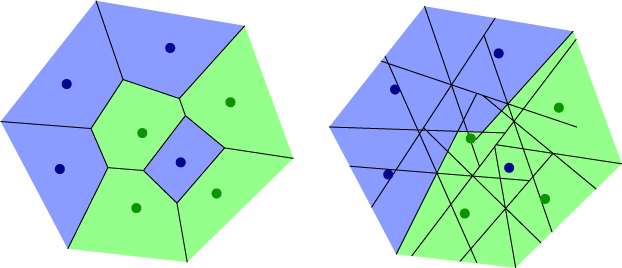
\includegraphics[width=0.9\textwidth]{knn1}
\label{fig:knn1}  

\end{figure}

\subsection{Árvore de Decisão}



Em sua forma mais simples, árvores de decisão são uma classe de algoritmos que buscam (no caso de classificação) achar a classe de um ponto de treino testando intervalos de suas \textit{features}. Vejamos o exemplo de uma árvore treinada a seguir:


\begin{figure}[ht]
	\centering
	\caption{Árvore de Decisão para prever a sobrevivência de passageiros do Titanic}
  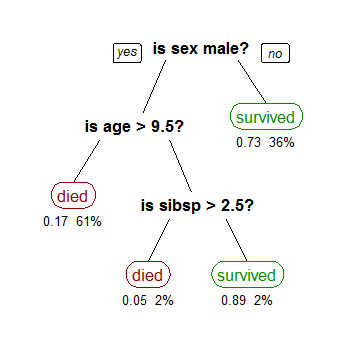
\includegraphics[width=0.9\textwidth]{tree1}
\label{fig:tree1}  

\end{figure}

Essa árvore busca prever se um determinado passageiro do Titanic sobreviveu ou não ao acidente testando diversas características desse indivíduo. Por exemplo, podemos ver que caso o sexo do passageiro seja feminino, ela tem uma alta chance de ter sobrevivido. Caso contrário, já são testadas outras duas cláusulas referentes a idade ao número de familiares também a bordo do navio. Por construção, temos um \textit{trade-off} para árvores, podendo trocar \textbf{legibilidade} por \textbf{precisão} (menos \textit{bias}). É possível construir árvores mais complexas que poderão a sua facilidade de interpretação por uma pessoa, porém poderão se adequar melhor ao dados treinados, e é essa ideia que é explorada por algoritmos de \textit{ensemble learning} como \textit{Random Forests} ou \textit{Adaboost}, que serão explicados em outra parte desse documento, mas que basicamente combinam o poder de diversas árvores treinadas iterativamente, para aumentar seu poder de classificação.


\subsection{Support Vector Machines}

Essa classe de algoritmos busca, para um conjunto de dados N-dimensionais, encontrar um hiperplano que separa o espaço dos dados em regiões de classificação. Vejamos um exemplo simples a seguir:


\begin{figure}[H]
	\centering
	\caption{SVM aplicado para classificar dados linearmente separáveis}
  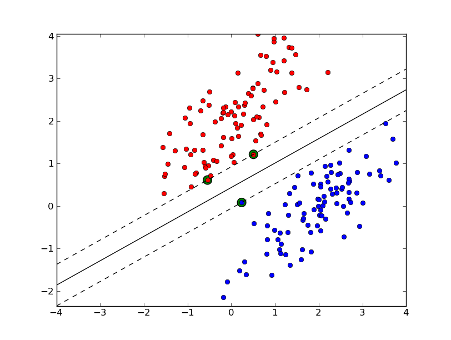
\includegraphics[width=0.8\textwidth]{svm1}
\label{fig:svm1}  

\end{figure}



A reta na figura \ref{fig:svm1} foi encontrada de modo a separar o espaço de classificação da classe "azul" do espaço de classificação da classe "vermelha". A linha pontilhada representa a margem de classificação, o algoritmo busca chegar a um hiperplano que tenha ainda uma distância dos pontos mais próximos da região de separação. A seguir, um exemplo mais complexo usando um \textit{kernel}  para poder classificar dados não linearmente separáveis:

\begin{figure}[H]
	\centering
	\caption{SVM aplicado para classificar dados de maneira não linear}
  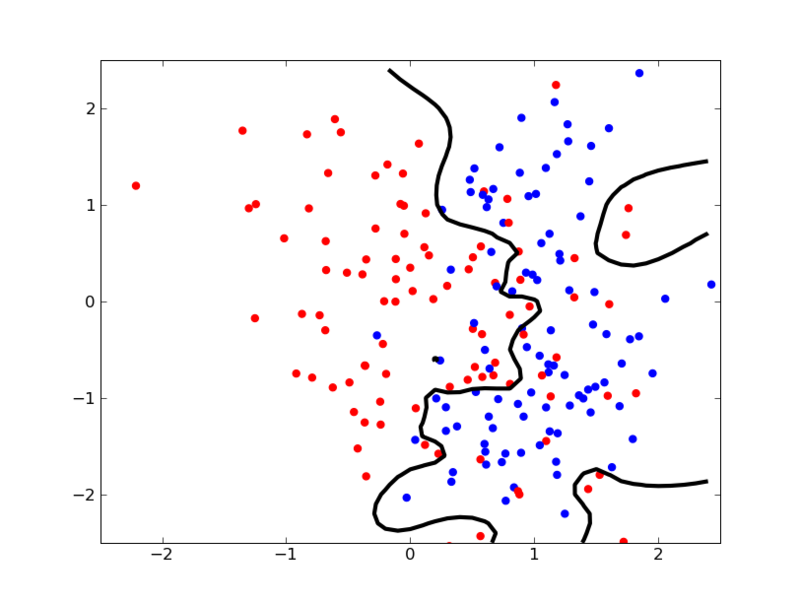
\includegraphics[width=0.8\textwidth]{svm2}
\label{fig:svm2}  

\end{figure}

\section{Aplicação na Prática}

No estudo e desenvolvimento da pesquisa, foi decidido finalmente combinar esses três algoritmos. Usaremos as conclusões levantadas por \cite{comparativeEN}, onde foi averiguado empiricamente que: 

\begin{enumerate}
\item Combinar as saídas de diversos classificadores pode reduzir o risco de selecionar um único que possa funcionar mal naquele caso específico
\item Os erros cometidos advindos de um classificador são geralmente compensados pela classificação correta de outro algoritmo no conjunto, de modo que a taxa de acerto \textit{do sistema} melhore
\item Classificadores base devem ser diversos em natureza para que a desição final não sofra de \textit{bias}
\end{enumerate}



